 \documentclass[12pt]{article}
\usepackage{polski}
\usepackage[utf8]{inputenc}
\usepackage{graphicx}
\usepackage{listings}
\usepackage{color}

\definecolor{dkgreen}{rgb}{0,0.6,0}
\definecolor{gray}{rgb}{0.5,0.5,0.5}
\definecolor{mauve}{rgb}{0.58,0,0.82}

\lstset{frame=tb,
  aboveskip=3mm,
  belowskip=3mm,
  showstringspaces=false,
  columns=flexible,
  basicstyle={\small\ttfamily},
  numbers=none,
  numberstyle=\tiny\color{gray},
  keywordstyle=\color{blue},
  commentstyle=\color{dkgreen},
  stringstyle=\color{mauve},
  breaklines=true,
  breakatwhitespace=true,
  tabsize=3
}


\begin{document}

\begin{titlepage}
\centering

\includegraphics[width=0.15\textwidth]{logo}\par\vspace{1cm}
{\scshape\LARGE Politechnika Warszawska \par}
\vspace{1cm}
{\huge\bfseries  Dokumentacja końcowa \linebreak \\  Chess Master\par}
\vspace{1cm}
{\bfseries Projekt Indywidualny \par}
\vspace{2cm}
{\Large\itshape  Sebastian Kurpios \par}
\end{titlepage}

\tableofcontents
\newpage

\section{Opis aplikacji}
Aplikacja Chess Master jest to program do gry w szachy z wykorzystaniem interfejsu 3D. Program pozwala na grę wieloosobową, obecnie z wykorzystaniem jednego komputera, lecz w przyszłości stanie się on również platformą webową. Ponadto program umożliwia komunikację pomiędzy graczami. Aplikacja jest zgodna ze standardami gry w szachy, a wykonane ruchy wyświetlają się w \textit{szachowej notacji algebraicznej}.
   
\section{Technologia wykonania}
Wykorzystane technologie:
\begin{itemize}
\item język programowania - C\#
\item GUI - Windows Forms, WPF
\item Interfejs 3D - Helix Toolkit
\end{itemize}   
   
\section{Wymagania}
Z powodu napisania aplikacji w technologii \textit{.NET}, do poprawnego działania aplikacji potrzebny jest system operacyjny Windows od wersji \textit{XP}. \\
Zalecane wymagania sprzętowe:
\begin{itemize}
\item procesor: min. 2 rdzeniowy, np. Intel Core 2 Duo
\item pamięć RAM: min. 1 GB
\item pamięć procesora GPU: 1 GB
\end{itemize}

\newpage
\section{Opis interfejsu}
\subsection{Menu}

\begin{figure}[!ht]
  \centering
	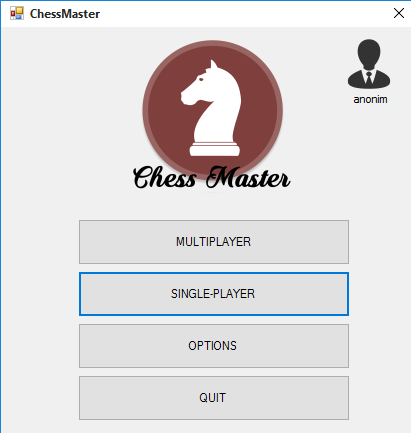
\includegraphics[scale=0.60]{interfejs1}
  \caption{Menu}
\end{figure}

Opis intefejsu (od góry):
\begin{itemize}
\item nazwa i zdjęcie użytkownika - po naciśnięciu otwiera okno edycji profilu lub logowania/rejestracji w przypadku braku zalogowania
\item Multiplayer - umożliwia grę wieloosobową
\item Single-player - umożliwia grę jednoosobową (obecnie opcja jest niedostępna)
\item Options - zawiera możliwy wybór opcji
\item Quit - umożliwia wyjście z aplikacji
\end{itemize}
\newpage
\subsection{Główny interfejs}

\begin{figure}[!ht]
  \centering
	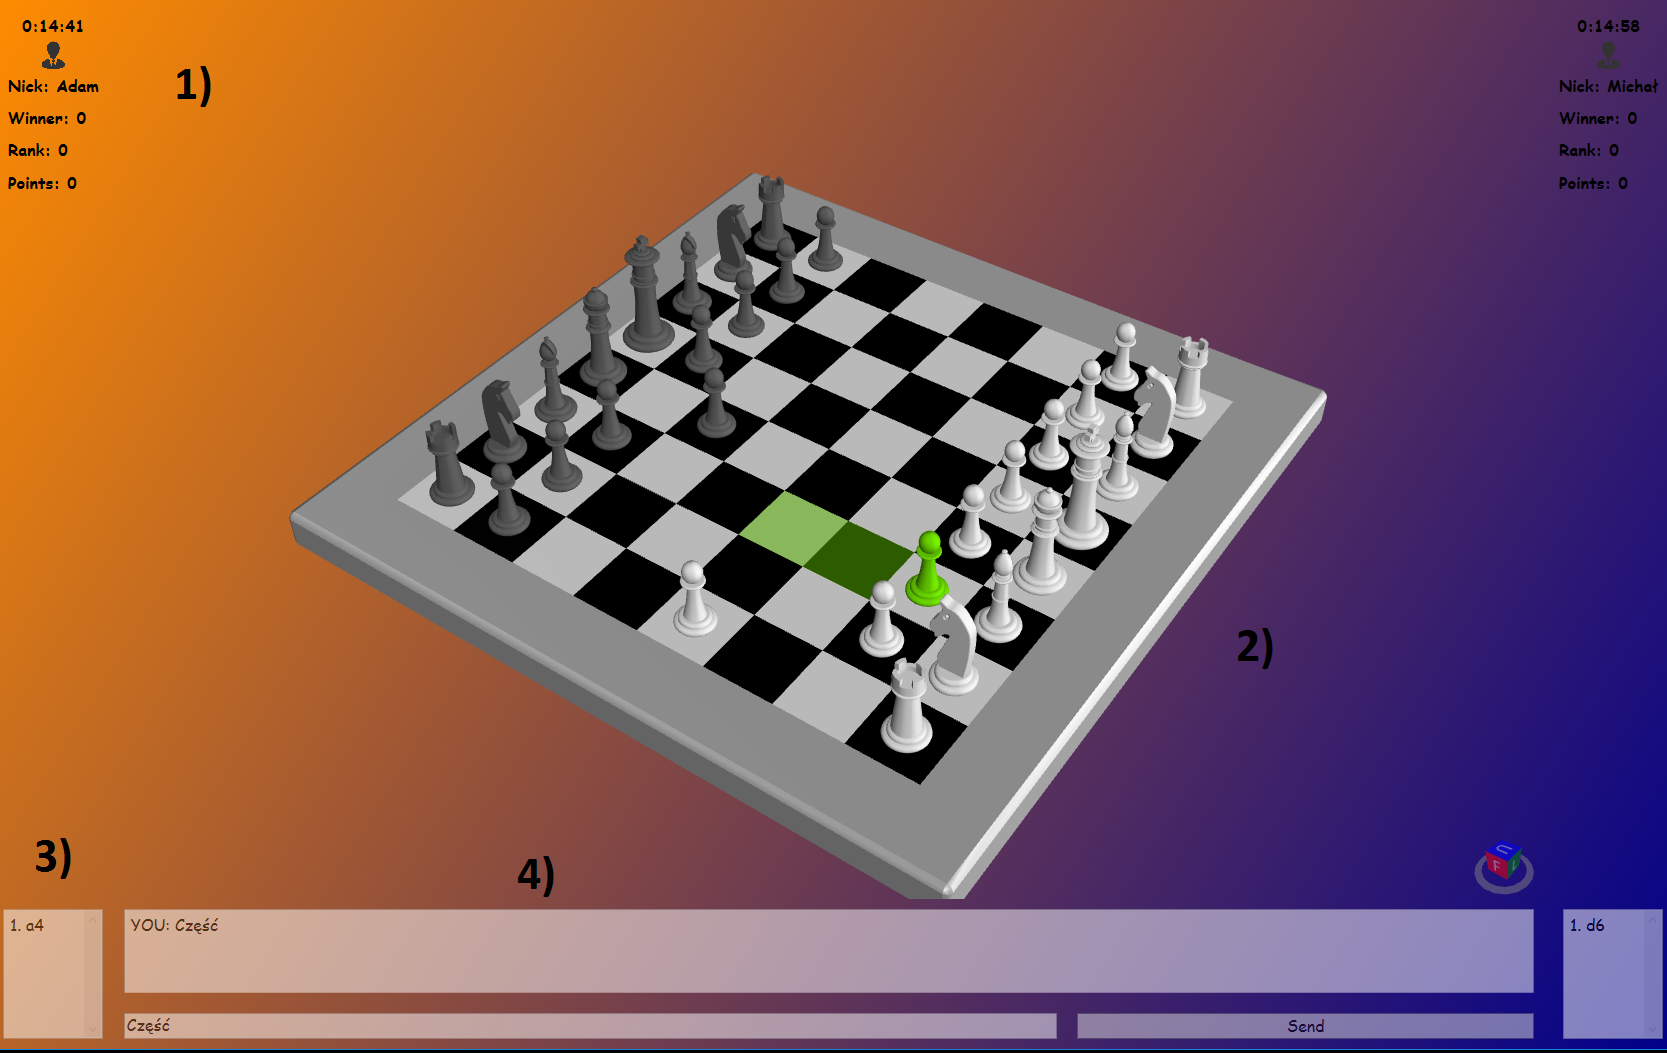
\includegraphics[scale=0.30]{interfejs2}
  \caption{Szachownica}
\end{figure}

Opis intefejsu (wg numerku):
\begin{enumerate}
\item pozostały czas oraz profil użytkownika - zdjęcie, liczba wygranych, liczba punktów, ranking; jeśli czas nie został podany to wyświetla czas gry użytkownika
\item plansza - po naciśnięciu na pionek użytkownika podświetlają się możliwe do wykonania ruchy (na zielono lub na czerwono w przypadku istnienia pojedynku lub ruchu specjalnego (roszada, bicie w przelocie)), naciśnięcie na podświetlane pole przenosi pionek na naciśnięty kwadrat
\item historia ruchów - pokazuje historię ruchów użytkownika w notacji algebraicznej
\item czat - umożliwia komunikację pomiędzy użytkownikami
\end{enumerate}
\newpage
\subsection{Interfejs logowania}

\begin{figure}[!ht]
  \centering
	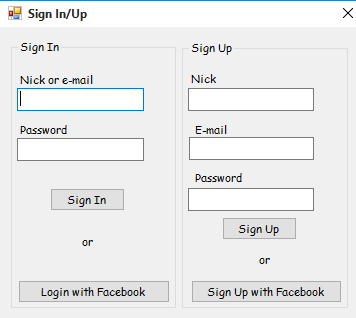
\includegraphics[scale=0.60]{interfejs3}
  \caption{Logowanie}
\end{figure}

Interfejs logowania umożliwia logowanie lub rejestrację. W tym celu wypełniamy formularz i naciskamy przycisk \textit{Sign In} lub \textit{Sign Up}.
Ponadto w przyszłości będzie możliwe logowanie się i rejestracja korzystając z serwisu \textit{facebook}.

\subsection{Interfejs edycji profilu}

\begin{figure}[!ht]
  \centering
	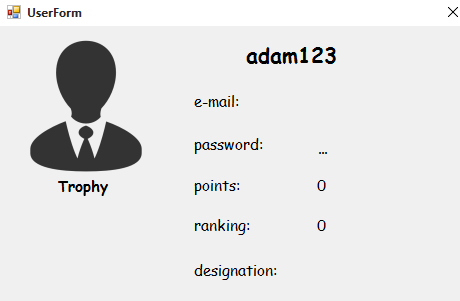
\includegraphics[scale=0.60]{interfejs4}
  \caption{Edycja profilu}
\end{figure}

Zawiera podstawowe informacje o użytkownku:
\begin{enumerate}
\item adres e-mail - możliwość zmiany
\item hasło - możliwość zmiany
\item liczba punktów
\item ranking
\item trofea i nagrody
\item zdjęcie profilowe - możliwość zmiany
\end{enumerate}

\end{document}